\section{Finite Element Machine}
\label{s.fema}

In this section, we present the Finite Element Machine classifier, as well as how it can cope with the problem of supervised pattern classification efficiently. \textcolor{blue}{In this point is import highlight that FEMa is not a generalization of the variation o k-NN (k-Nearest Neighbour) or w-NN (Weighted Nearest Neighbour)~\cite{Samworth:12} even w-NN can being seen as an special case of the FEMa. So it is very important emphasize that FEMa has all fundamental background based on Finite Element Method . The FEMa allows work with a huge number of different basis, as: Radial Basis Function, Normalized Radial Basis Function and many others. All the background developed in this work provides a elegant solutions for basis which are neither interpolating and not partition-unit basis.  FEMa opens a wide range of new studies of finite element bases applied in machine learning.}

\subsection{Background Theory}
\label{ss.background}

Let ${\cal Z}={\cal Z}_1\cup{\cal Z}_2$ be a dataset partitioned into a training (${\cal Z}_1$) and a test (${\cal Z}_2$) set. In this case, the pair $(\textbf{x}_i,y_i)\in{\cal Z}$ denotes the feature vector $\textbf{x}_i\in\Re^m$ extracted from sample $i$, and $y_i$ stands for its label. Notice we adopted the very same formulation used in the previous section, i.e. a point in FEM formulation stands for a sample in FEMa.

Roughly speaking, FEMa learns a set of probability functions ${\cal P}(\textbf{x})=\{P_1(\textbf{x}),P_2(\textbf{x}),\ldots,P_c(\textbf{x})\}$, where $c$ stands for the number of classes, and $P_i(\textbf{x})$ represents the probability of a given sample $\textbf{x}$ to be assigned to class $i$. In other words, FEMa aims at learning a probabilistic manifold from the training set.

\subsection{Probabilistic Manifold Learning}
\label{ss.manifold}

Depending on the basis function used to interpolate points, FEMa does not require a training step, which turns out to be quite interesting when dealing with big data. Precisely, this assumption is true concerning bases that are natively interpolating, such as Shepard basis. On the other hand, with respect to non-interpolating basis, e.g. radial functions, one needs to compute $\textbf{Z}^{-1}$ in Equation~\ref{e.interpolating_basis}. Also, if the basis function does not hold the partition of unity property, one shall compute Equation~\ref{e.normalization} either. Therefore, although FEMa can be used with any basis function, we shed light over that bases holding both the interpolating and partition of unity properties are much more appealing when dealing with massive amount of data. As such, we can consider the calculation of $\textbf{Z}^{-1}$ and Equation~\ref{e.normalization} as the training steps when using non-interpolating and non-partition of units bases.

Assuming we are using an interpolating and partition of unity basis (e.g Shepard), we can move to the classification step. Given a sample $\textbf{x}\in{\cal Z}_2$, we need to compute its probability of belonging to each class $i$, $i=1,2,\ldots,c$, as follows:

\begin{equation}
	P_i(\textbf{x})=\sum_{j=1}^{\left|{\cal Z}_1\right|}\rho_i^j\phi_j(\textbf{x}),
\end{equation}
where $\rho_i^j\in[0,1]$ stands for the probability of training sample $j$ belonging to class $i$. An interesting property concerning FEMa relates to the possibility in assigning a probability to each training sample, which means we have an uncertainty associated to those samples, thus having an important role when dealing with data overfitting. This capability is extremely important in medical-driven applications, where physicians usually have different opinions with respect to the very same data (e.g. cancer detection in images).

The probability $\rho_i^j\in[0,1]$ can be computed using the following formulation:

\begin{equation}
\rho_i^j =  \left\{
			  \begin{array}{ll}
			      1 & \hbox{if $y_{j} = i$}\\
			      0 & \hbox{otherwise.}\\
			  \end{array}
		    \right.
\end{equation}
Since we have labeled datasets (i.e. we are assuming the labeling process is errorless), we can use $\rho_i^j\in\{0,1\}$. Therefore, we generate the set of probabilities ${\cal P}(\textbf{x})$ for each sample $\textbf{x}\in{\cal Z}_2$. 

In short, FEMa classifies a given sample $\textbf{x}\in{\cal Z}_2$ as belonging to the class $\hat{y}$ that satisfies the above equation:

\begin{equation}
	\hat{y} = \arg\max_{i}P_i(\textbf{x}).
\end{equation}
Also, FEMa allows us to infer the certainty $C(\textbf{x})$ as follows:

\begin{equation}
\label{eq.certainty}
	C(\textbf{x})=\frac{P_{\hat{y}}(\textbf{x})}{\sum_{j=1}^cP_j(\textbf{x})}.
\end{equation}
Therefore, FEMa can produce both hard and soft (probability) outputs without any modification. Figure~\ref{fig.ProbFunc} illustrates the process of learning the probability functions of each class in a one-dimensional and two-class problem. For the sake of explanation, the $x$-axis stands for a test set with samples within the interval $[-3,3]$, and the $y$-axis denotes their probability values with respect to the class $1$ (Figure~\ref{fig.ProbFunc}a) and class $2$ (Figure~\ref{fig.ProbFunc}b). Also, the red dots stand for the training samples, i.e. the centers of the basis functions.

Let us consider a test sample with value $-2$ in Figure~\ref{fig.ProbFunc}c. As one can observe, such sample has been used as a center for the basis function in Figure~\ref{fig.ProbFunc}a already (it is a training sample). In this case, the classification process will assign class $1$ to this sample, since $P_1(-2)\approx 1$, and $P_2(-2)\approx 0$. Now, consider a sample with value $2$ that does not belong to the training set, i.e. it is not a basis center. In this case, $P_1(2)\approx 0.15$ and $P_2(2)\approx 0.85$, which leads FEMa to assign class $2$ to that sample.

\begin{figure}[!htb]
\centering
\begin{tabular}{cc}
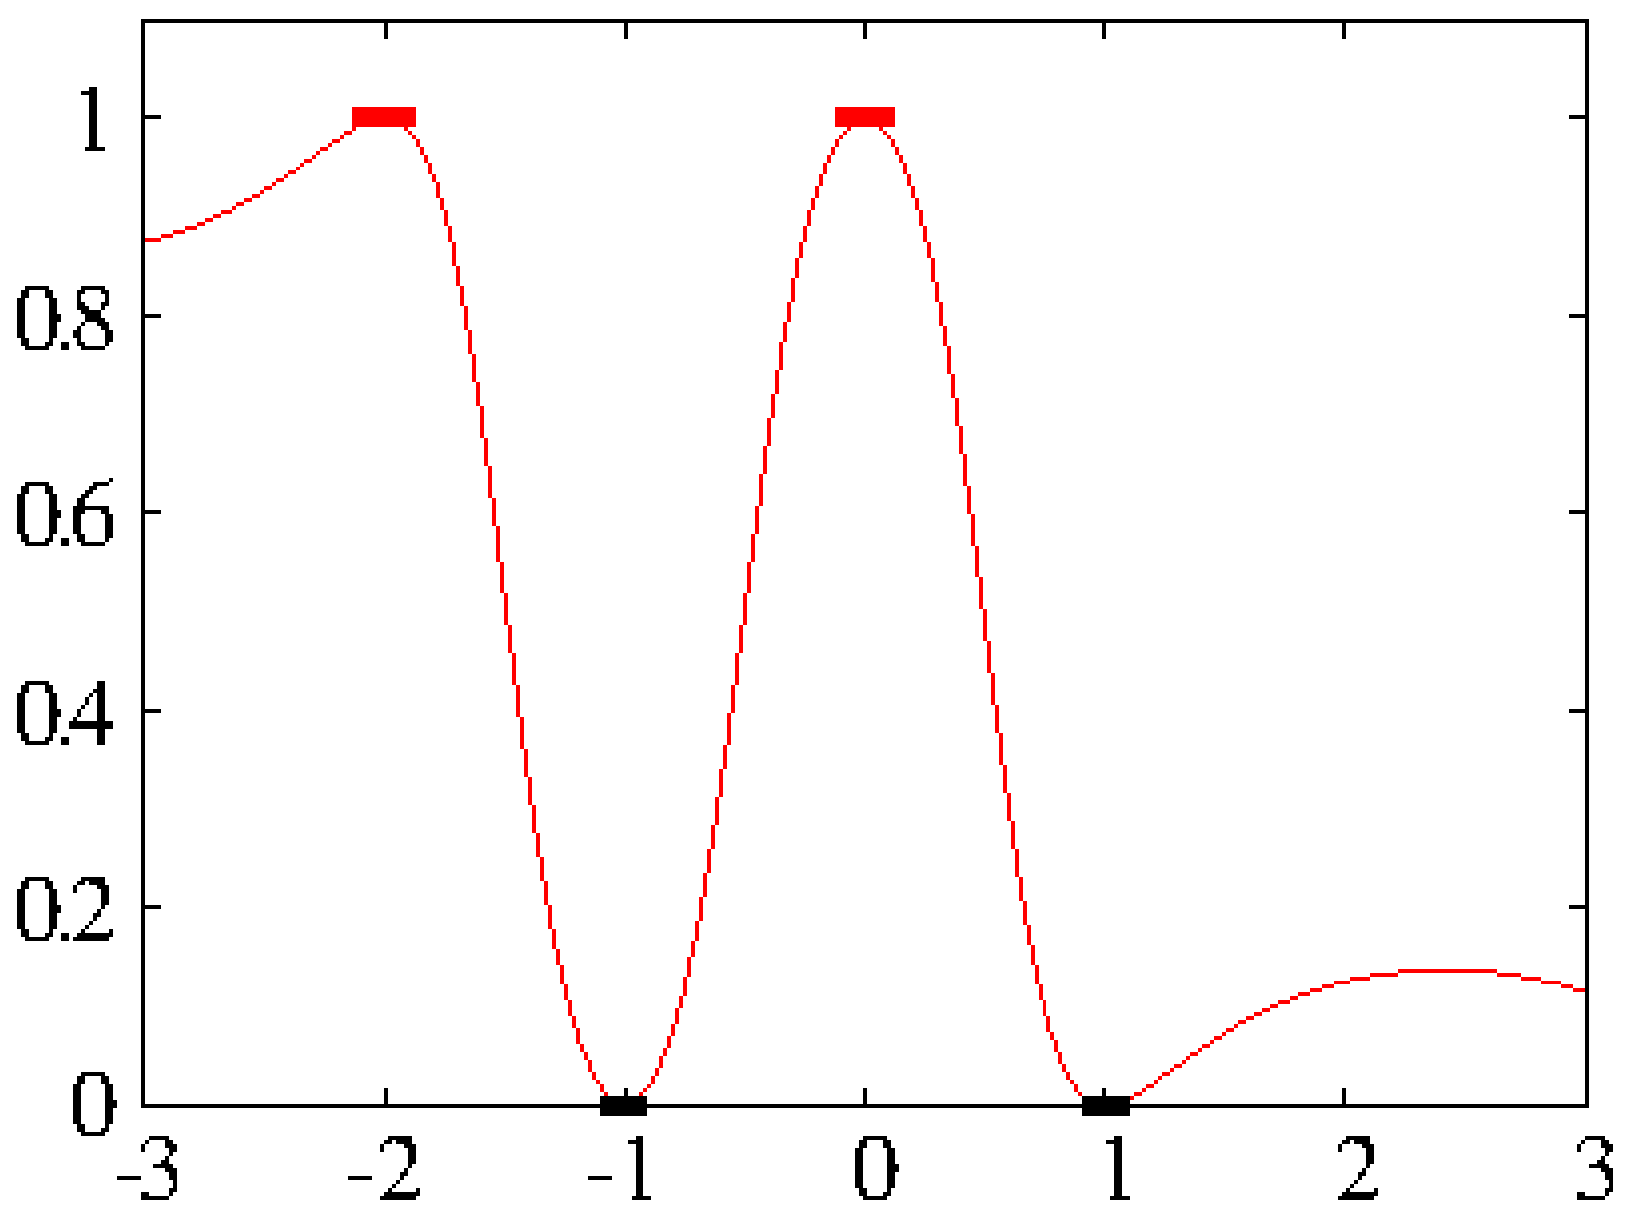
\includegraphics[scale=0.153]{./ShepardClass1.eps} &
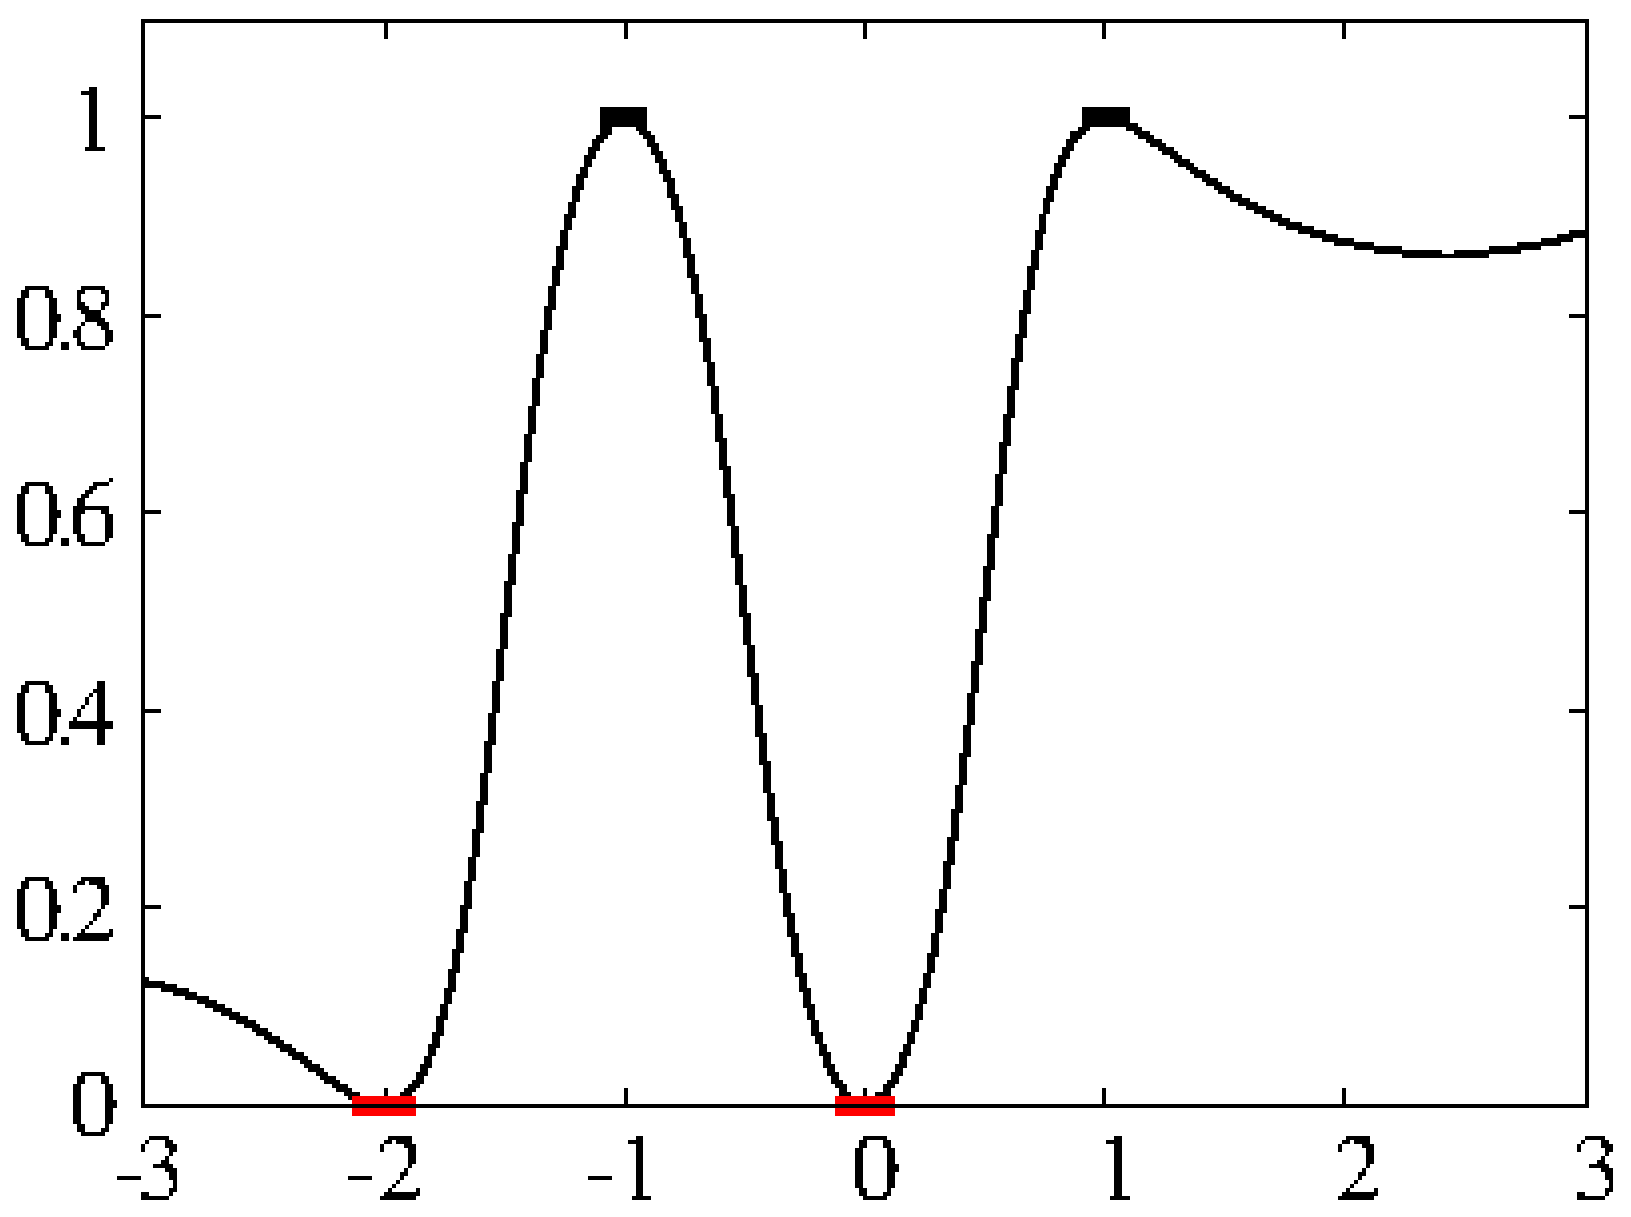
\includegraphics[scale=0.153]{./ShepardClass2.eps} \\
(a) & (b)\\
\end{tabular}
\begin{tabular}{c}
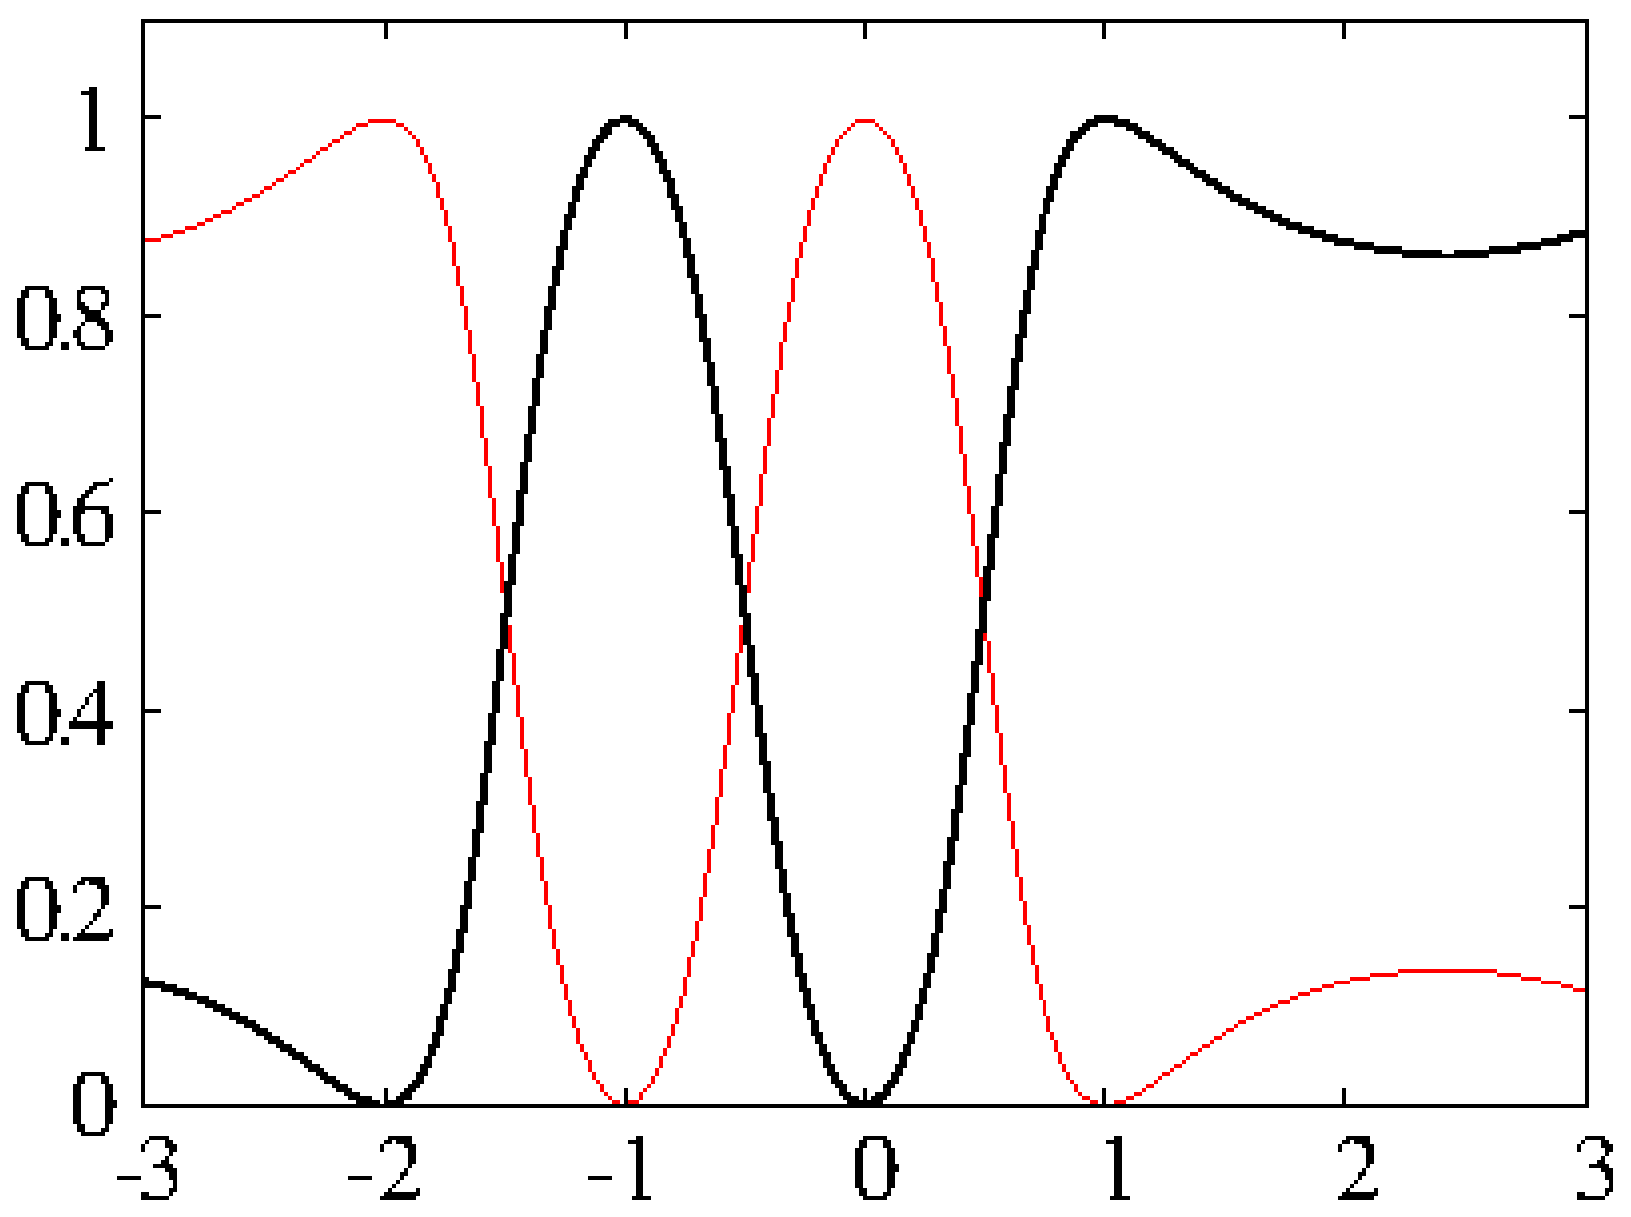
\includegraphics[scale=0.153]{./ShepardProbClass.eps} \\
(c)
\end{tabular}
\caption{The Shepard approximation of the probability function of a two-class problem using $k=3$ considering a given sample $\textbf{x}$: (a) $P_1(\textbf{x})$ and (b) $P_2(\textbf{x})$. The red dots and the red curve denote the samples and the probability function of class $1$, respectively, and the black dots and the black curve stand for the samples and the probability function of class $2$, respectively. In (c), we have the two probability functions together. Notice each real number in $[-3,3]$ (i.e. $x$-axis) is classified according to the class that has the higher probability value (i.e. $y$-axis).}
\label{fig.ProbFunc}
\end{figure}

\subsection{Toy Example}
\label{ss.toy}

In this section, we present the FEMa working mechanism on a bidimensional classification problem. Figure~\ref{2Dpoints}a shows a training set with samples distributed over three classes (red, green and blue). The task is to verify the influence region of each training sample in the image domain, i.e. to classify the remaining points (white ones) in the image frame displayed in Figure~\ref{2Dpoints}a. In this case, the feature of each sample (point) is just its $(x,y)$-position.

\begin{figure}[!htb]
\centering
\begin{tabular}{cc}
\hspace{0.31cm}\moldura{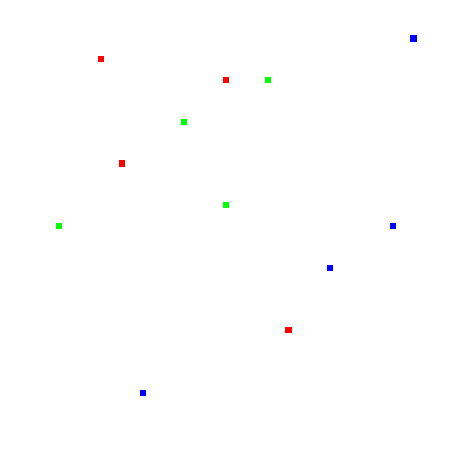
\includegraphics[width=3.39cm]{./points.eps}} &
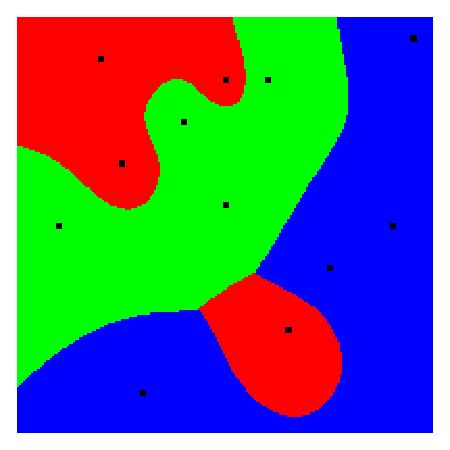
\includegraphics[width=3.39cm]{./out_p1.eps} \\
(a) & (b)\\
\end{tabular}\newline
\begin{tabular}{cc}
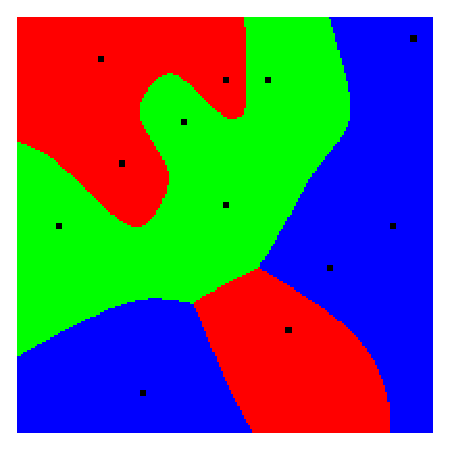
\includegraphics[width=3.39cm]{./out_p3.eps} &
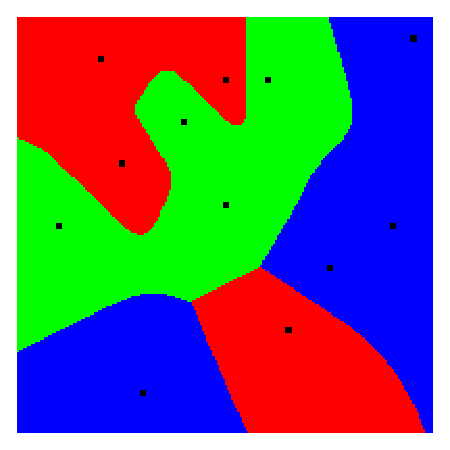
\includegraphics[width=3.39cm]{./out_p5.eps} \\
(c) & (d)\\
\end{tabular}
\caption{FEMa working mechanism: (a) training set with samples distributed in three classes, and the image classified by FEMa using (b) $k=1$, (c) $k=3$ and (d) $k=5$.}
\label{2Dpoints}
\end{figure}

Figures~\ref{2Dpoints}b,~\ref{2Dpoints}c and~\ref{2Dpoints}d depict the image frame classified by FEMa using the Shepard basis with $k=1$, $k=3$ and $k=5$, respectively. Since we are using the $(x,y)$ coordinates to describe each sample, the labeled image refers to the influence region of each training sample, which ends up generating the boundaries of each class. Notice that FEMa can obtain quite good and smooth decision boundaries for different values of $k$ (Equation~\ref{eq.w}). As matter of fact, the larger the value of $k$, the less points will influence the interpolating process of the probability function. For the sake of clarification purposes, when $k\to\infty$, FEMa tends to behave similarly to the well-known nearest neighbor classifier.

Figure~\ref{fig.2Dcertain}a displays the degree of certainty (Equation~\ref{eq.certainty}) computed by FEMa with $k=3$ for each test sample with respect to Figure~\ref{2Dpoints}a. The brighter the pixel, the greater its degree of certainty to be assigned to some class. Notice the darker pixels fall in the boundary among classes (Figure~\ref{2Dpoints}c). Figure~\ref{fig.2Dcertain}b represents each test sample by its label color weighted by its degree of certainty.

\begin{figure}[!htb]
\centering
\begin{tabular}{cc}
 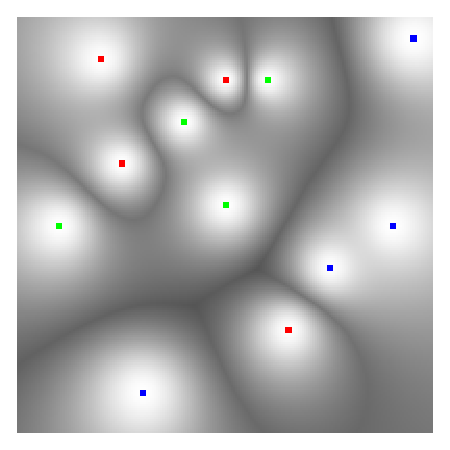
\includegraphics[scale=0.5]{./certain_p.eps} &
 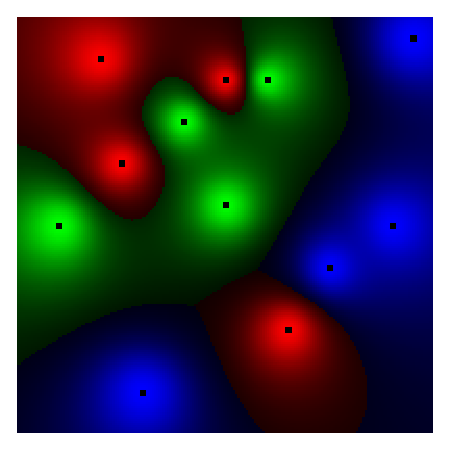
\includegraphics[scale=0.5]{./out_w_p.eps} \\
 (a) & (b)
 \end{tabular} 
 \caption{Probability map (degree of certainty) computed by FEMa in (a), and the test samples with their class label weighted by their respective degree of certainty.}
   \label{fig.2Dcertain}
\end{figure}

\subsection{Complexity Analysis}
\label{ss.complexity}

As aforementioned, depending on the basis function used to build the probabilistic manifold (i.e. interpolating and partition of unity properties), FEMa does not require an explicit training step, since we just need to place the training points, thus taking $\theta(1)$. However, if one uses a non-interpolating basis function, we need to compute the inverse matrix $\textbf{Z}^{-1}$ in Equation~\ref{e.interpolating_basis}, which requires $\theta(\left|{\cal Z}_1\right|^{2.37})$ using the Coppersmith-Winograd algorithm~\cite{Coppersmith:90}.

In regard to the classification phase, for each test sample $\textbf{x}$, we need to compute Equation~\ref{eq.shepard_basis}, which requires $\theta({\left|{\cal Z}_1\right|})$. However, the denominator of such equation considers all training samples, thus becoming a constant, and we need to compute it only once. Since the test set contains $\left|{\cal Z}_2\right|$ samples, the overall classification phase takes $\theta(\left|{\cal Z}_1\right|+\left|{\cal Z}_1\right|\left|{\cal Z}_2\right|)\in\theta(\left|{\cal Z}_1\right|.\left|{\cal Z}_2\right|)$. Therefore, by using an interpolating basis function, the whole FEMa learning and classification processes require a quadratic complexity with respect to the training/testing set size (i.e. when $\left|{\cal Z}_1\right|=\left|{\cal Z}_2\right|$).

However, when we have unbalanced datasets, samples from the majority classes will have a stronger influence when computing the probability functions. Suppose a two-class classification problem, i.e. we have samples from the positive and negative samples. Also, suppose samples from the negative class comprise only $1\%$ of the number of positive samples. When we are computing the probability function of test sample, the positive samples will play a major role during this computation process. In order to overcome this problem, we can use only the $T$ nearest training samples from each class, where $T\in O(\alpha)$ and $\alpha$ stands for the number of elements from the smallest class\footnote{In this paper, we use $T=\alpha$.}. In this case, since we need to sort the training samples according to their distances for each test sample, the classification phase now takes $\theta((\left|{\cal Z}_1\right|\log\left|{\cal Z}_1\right|).\left|{\cal Z}_2\right|)$. Notice we can make it better by using some special data structures, such as kd-trees, which require $\theta(\left|{\cal Z}_1\right|\log\left|{\cal Z}_1\right|)$ for loading the whole data only once during training. Now, with respect to the classification phase, we do not need the sorting step, since to obtain the nearest $T$ samples takes $O(T.\log\left|{\cal Z}_1\right|)$, and thus the classification phase requires $\theta((T.\log\left|{\cal Z}_1\right|).\left|{\cal Z}_2\right|)$.